%% introduction.tex
%% Copyright 2023 TJ-CSCCG
%
% This work may be distributed and/or modified under the
% conditions of the LaTeX Project Public License, either version 1.3
% of this license or (at your option) any later version.
% The latest version of this license is in
%   http://www.latex-project.org/lppl.txt
% and version 1.3 or later is part of all distributions of LaTeX
% version 2003/12/01 or later.
%
% This work has the LPPL maintenance status "maintained".
%
% This Current Maintainer of this work is Rizhong Lin.
%
% This work consists of all the *.tex and *.sty files in
%   https://github.com/TJ-CSCCG/Tongji-Beamer
\section{项目背景}

\begin{frame}{项目背景}
    \small
    \begin{block}{项目背景}
        \begin{itemize}
            \item 软件测试设计往往依赖人工从需求中抽取覆盖项、风险点与测试策略，成本高且一致性不足。
            \item FitnessAI 同时包含姿态分析、状态机计数、记录过滤、统计聚合等多类业务逻辑，适合作为测试设计工具的验证对象。
            \item 因此我们实现 AutoTestDesign，将需求分析、风险评估、测试设计与交互审查串成一条完整工作流。
        \end{itemize}
    \end{block}
\end{frame}

\begin{frame}{项目目标}
    \small
    \begin{block}{项目目标}
        \begin{itemize}
            \item 构建一个可运行的 AI 驱动测试设计工具，支持需求结构化、QRA、黑盒/白盒设计与导出。
            \item 使用该工具测试 FitnessAI 项目。
            \item 通过自动化执行、Allure 报告和 JaCoCo 覆盖率验证工具输出的有效性。
        \end{itemize}
    \end{block}

    \begin{block}{整体方案}
        \begin{itemize}
            \item 工具：AutoTestDesign（Vue 3 + Express + FastAPI + PostgreSQL）
            \item 目标应用：FitnessAI 智能健身辅助系统
            \item 验证路径：QRA 风险分析 -> 测试计划 -> 详细测试设计 -> 自动化执行与覆盖率证据
        \end{itemize}
    \end{block}
\end{frame}

\begin{frame}{项目范围与产出}
    \begin{columns}[T]
        \column{0.42\textwidth}
        \footnotesize
        \begin{itemize}
            \item 目标接口：
            \item \texttt{/api/analytics/pose}
            \item \texttt{/api/user/\{id\}/records}
            \item \texttt{/api/user/\{id\}/dashboard}
            \item 扩展范围：记录筛选、\texttt{/api/exercises}、reset 接口
            \item 工具输出：10 条结构化需求、10 条风险项、37 个覆盖项、81 条测试用例、6 种设计方法
            \item 验证证据：Markdown / JSON / CSV / Excel + JUnit 5 + Allure + JaCoCo
        \end{itemize}

        \column{0.54\textwidth}
        \begin{figure}
            \centering
            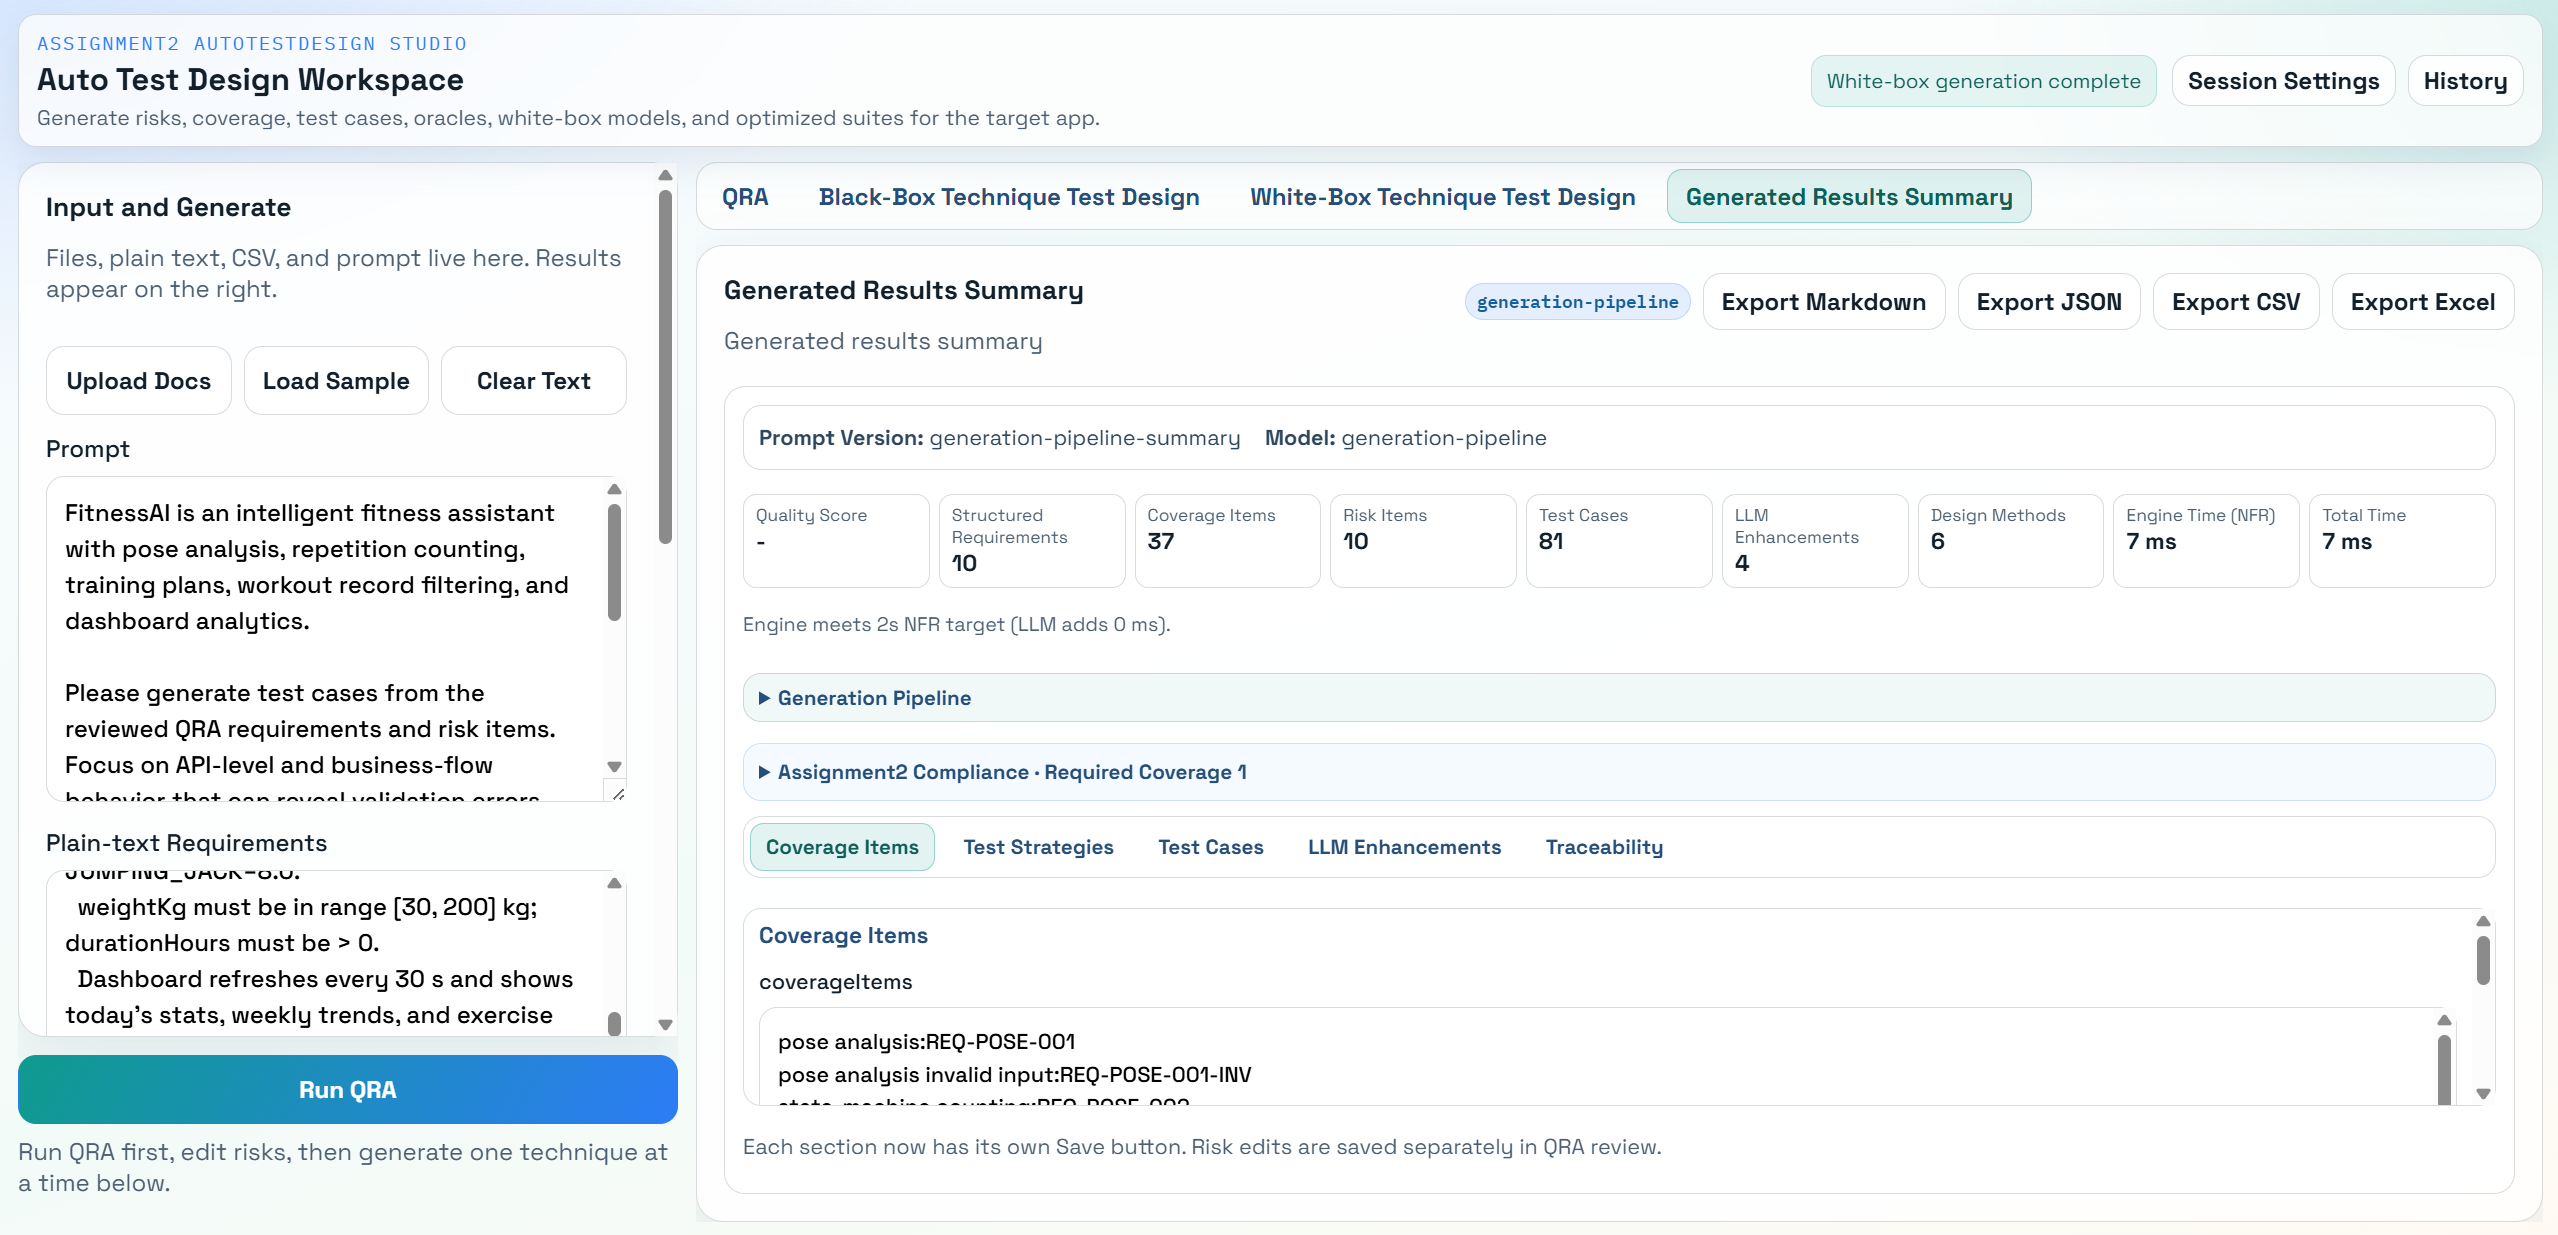
\includegraphics[width=0.98\textwidth]{contents/figure/fitnessai/Summary.png}
        \end{figure}
    \end{columns}
\end{frame}
